%----------------------------------------------------------------------------------------
%    PACKAGES AND THEMES
%----------------------------------------------------------------------------------------

\documentclass[aspectratio=169,xcolor=dvipsnames]{beamer}
\usetheme{SimplePlus}

\usepackage{tikz}
\usepackage{hyperref}
\usepackage{graphicx} % Allows including images
\usepackage{booktabs} % Allows the use of \toprule, \midrule and \bottomrule in tables
\usepackage{wrapfig}
\usepackage{listings}
\usepackage[font=small,labelfont=bf]{caption}

%----------------------------------------------------------------------------------------
%    TITLE PAGE
%----------------------------------------------------------------------------------------

\title{Tree-Based Methods}
\subtitle{HI 743}

\author{Ryan Gallagher}

\institute
{
    Department of Health Informatics and Administration \\
    Zilber College of Public Health \\
    University of Wisconsin - Milwaukee% Your institution for the title page
}
\date{March 13th, 2025} % Date, can be changed to a custom date


%----------------------------------------------------------------------------------------
%    PRESENTATION SLIDES
%----------------------------------------------------------------------------------------

\begin{document}
\begin{frame}
    % Print the title page as the first slide
    \titlepage
\end{frame}

%----------------------------------------------------------------------------------------
%    Outline
%----------------------------------------------------------------------------------------

\begin{frame}{Overview}
    % Throughout your presentation, if you choose to use \section{} and \subsection{} commands, these will automatically be printed on this slide as an overview of your presentation
    \tableofcontents
\end{frame}

%----------------------------------------------------------------------------------------
%    Slides
%----------------------------------------------------------------------------------------
% Slide: Introduction to Decision Trees
\section{Regression Trees}
\begin{frame}{Introduction to Decision Trees}
    \begin{itemize}
    	\setlength\itemsep{0.5cm}
        \item Tree-based methods are non-parametric approaches used for both classification and regression tasks.
        \item They partition the feature space into distinct regions and make predictions based on the majority class (classification) or average response (regression).
        \item Decision trees provide an intuitive and interpretable way to model relationships between variables.
    \end{itemize}
\end{frame}

% Slide: Tree Structure and Terminology
\begin{frame}{Tree Structure and Terminology}
    \begin{itemize}
        \item Each split in the tree creates two branches, dividing the predictor space into regions.
        \item The final partitions are known as \textbf{terminal nodes} or \textbf{leaves}.
        \item Internal nodes define the decision rules based on feature values.
        \item The process of growing a tree continues until stopping criteria (such as minimum node size) are met.
    \end{itemize}
    \centering
    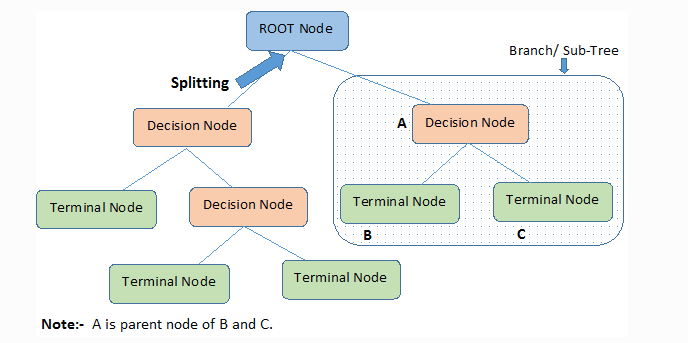
\includegraphics[width=0.6\textwidth]{images/terminology.png}
\end{frame}


% Slide: Regression Trees
\begin{frame}{Regression Trees}
    \begin{itemize}
        	\setlength\itemsep{0.5cm}
        \item Regression trees are used when the response variable is continuous.
        \item The predictor space is recursively split into distinct and non-overlapping regions.
        \item Each split is chosen to minimize the residual sum of squares (RSS) within each region.
        \item The predicted value for each region is the mean response of the training observations in that region.    \end{itemize}
    \begin{center}
        %\includegraphics[width=0.6\textwidth]{regression_tree_example.png}
    \end{center}
\end{frame}

\begin{frame}
\centering
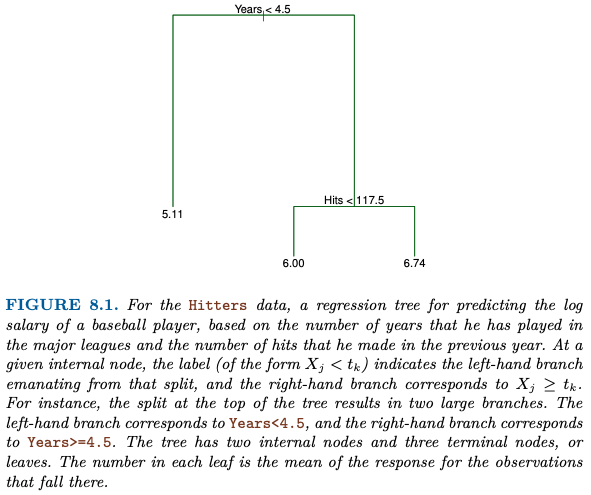
\includegraphics[scale = 0.45]{images/reg_tree.png}
\end{frame}

\begin{frame}
\centering
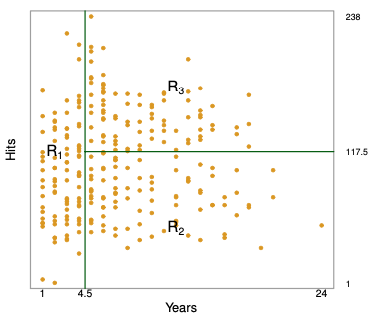
\includegraphics[scale = 0.65]{images/partition.png}
\end{frame}

\section{Tree Pruning}
% Slide: Tree Pruning
\begin{frame}{Tree Pruning}
    \begin{itemize}
        \item \textbf{Decision trees tend to overfit the training data}, resulting in high variance and poor generalization to unseen data.
        \item \textbf{Pruning} is a technique used to simplify trees by removing branches that do not improve predictive performance.
        \item \textbf{Cost complexity pruning} (also known as \textit{weakest link pruning}) selects a subtree that minimizes a balance between the RSS and tree complexity:
        \begin{equation}
            \sum_{m=1}^{|T|} \sum_{i: x_i \in R_m} (y_i - \hat{y}_{R_m})^2 + \alpha |T|
        \end{equation}
        \item The parameter \( \alpha \) controls the trade-off between model complexity and fit (tuning parameter).
    \end{itemize}
\end{frame}

% Slide: Types of Pruning
\begin{frame}{Types of Pruning}
    \begin{itemize}
    \setlength\itemsep{1cm}
        \item \textbf{Pre-pruning} (early stopping): Stops tree growth when a criterion is met (e.g., minimum number of observations in a node).
        \begin{itemize}
            \item Prevents overly complex trees but risks missing meaningful structure.
        \end{itemize}
        \item \textbf{Post-pruning} (cost complexity pruning): Grows a large tree and prunes back using cross-validation to select the best subtree.
        \begin{itemize}
            \item More computationally intensive but generally leads to better models.
        \end{itemize}
    \end{itemize}
\end{frame}

\section{Cross-Validation}
% Slide: Cross-Validation for Pruning
\begin{frame}{Cross-Validation}
    \begin{itemize}
        \item \textbf{Cross-validation} is a technique used to estimate model performance and avoid overfitting.
        \item The data is \textbf{split into multiple subsets} (folds), and the model is trained and tested across these folds.
        \item In pruning, cross-validation helps determine the optimal complexity parameter \( \alpha \) by selecting the subtree that minimizes prediction error.
        \item Common choices include \textbf{k-fold cross-validation} (e.g., 10-fold CV) to balance bias and variance.
    \end{itemize}
\end{frame}


\begin{frame}{Cross-Validation for Pruning \& Advantages}
\textbf{Cross Validation:}
    \begin{itemize}
        \item The optimal subtree is selected using cross-validation.
        \item A sequence of pruned trees is generated using different values of \( \alpha \).
        \item The tree minimizing the cross-validation error is selected.
    \end{itemize}
\textbf{Advantages of Pruning:}
    \begin{itemize}
        \item Reduces overfitting, leading to better generalization to unseen data.
        \item Produces simpler and more interpretable models.
        \item Reduces variance, improving stability of the predictions.
    \end{itemize}
\end{frame}

\section{Classification Trees}
% Slide: Classification Trees
\begin{frame}{Classification Trees}
    \begin{itemize}
    %\setlength\itemsep{0.5cm}
        \item Used for predicting categorical responses rather than continuous values.
        \item Each observation is assigned to the most common class in the corresponding terminal node.
        \item Provides both class predictions and class probabilities for interpretability.
        \item Recursive binary splitting is used to partition the feature space.
    \end{itemize}
    \centering
    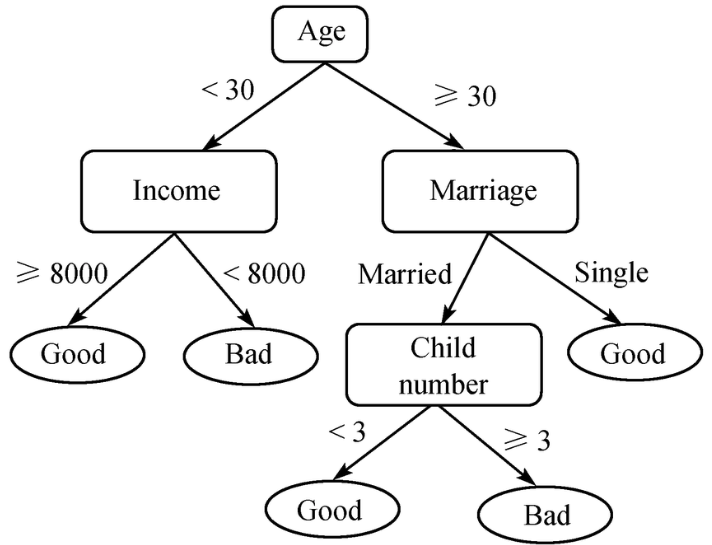
\includegraphics[width=0.33\textwidth]{images/class_tree.png}
\end{frame}

% Slide: Impurity Measures
\begin{frame}{Evaluation Measures for Classification Trees}
    \begin{itemize}
        \item \textbf{Classification Error Rate:} Measures misclassification frequency but is not sensitive enough for tree growth.
        \item \textbf{Gini Index:} Measures total variance across classes:
        \begin{equation}
            G = \sum_{k=1}^{K} \hat{p}_{mk} (1 - \hat{p}_{mk})
        \end{equation}
        \item \textbf{Entropy:} Measures uncertainty:
        \begin{equation}
            D = -\sum_{k=1}^{K} \hat{p}_{mk} \log \hat{p}_{mk}
        \end{equation}
        \item Both Gini Index and Entropy provide better sensitivity to node purity compared to classification error.
    \end{itemize}
\end{frame}

% Slide: Comparing Classification Methods
\begin{frame}{Comparing Classification Trees with Other Methods}
    \begin{itemize}
    \setlength\itemsep{0.5cm}
        \item Classification trees provide an intuitive and interpretable model.
        \item However, they tend to have higher variance and lower accuracy compared to ensemble methods.
        \item Alternative classification methods include:
        \begin{itemize}
            \item Logistic Regression (for linear decision boundaries)
            \item K-Nearest Neighbors (for non-linear decision boundaries)
            \item Support Vector Machines (for high-dimensional spaces)
        \end{itemize}
    \end{itemize}
\end{frame}

\begin{frame}
\begin{figure}
\centering
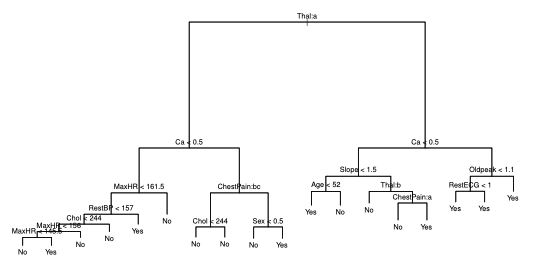
\includegraphics[scale = 0.65]{images/pruned_class.png}
\caption{Hitters Classification Tree (unpruned)}
\end{figure}
\end{frame}

\begin{frame}
\centering
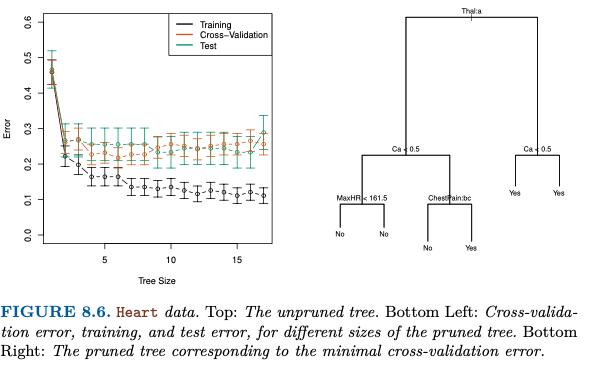
\includegraphics[scale = 0.6]{images/big_class.png}
\end{frame}

\section{Trees vs. Linear Models}
% Slide: Trees vs. Linear Models
\begin{frame}{Trees vs. Linear Models}
    \begin{itemize}
        \item Linear models assume a linear relationship:
        \begin{equation}
            f(X) = \beta_0 + \sum_{j=1}^{p} \beta_j X_j
        \end{equation}
        \item Trees partition the predictor space into regions and fit a constant in each region:
        \begin{equation}
            f(X) = \sum_{m=1}^{M} c_m \cdot 1(X \in R_m)
        \end{equation}
        \item Trees work well for capturing complex, nonlinear relationships, while linear models excel when a linear structure is appropriate.
    \end{itemize}
\end{frame}

% Slide: When to Use Trees vs. Linear Models
\begin{frame}{When to Use Trees vs. Linear Models}
    \begin{itemize}
    \setlength\itemsep{0.5cm}
        \item Use \textbf{linear models} when:
        \begin{itemize}
            \item The relationship between predictors and response is approximately linear.
            \item Interpretability and inferential understanding are important.
            \item The number of predictors is small and well-structured.
        \end{itemize}
        \item Use \textbf{decision trees} when:
        \begin{itemize}
            \item The relationship between predictors and response is highly nonlinear.
            \item There are complex interactions between features.
            \item Handling missing data and categorical variables directly is beneficial.
        \end{itemize}
    \end{itemize}
\end{frame}



\end{document}